\documentclass[Thesis.tex]{subfiles}
\begin{document}
\chapter{Machine Learning}
\label{chp:machine-learning}

Machine learning (ML) is a field of study concerned with building
models\footnote{The term \emph{model} is used in a very general sense, and
refers to anything that takes information as input and produces a corresponding
output.} that can perform a task without the need for explicit instructions of
how to do so. The key word is \emph{learning}; we want to enable the model to
discover the best way to solve the task at hand within the constraints that we
have imposed on it.

A simple example of a Machine Learning algorithm is linear regression, where we endeavor to
find a linear function that best fits some observed data, with respect to some
metric of what constitutes a \emph{good fit}. Other examples include
dimensionality reduction, image classification, algorithmic trading, playing
chess. Note that all of these examples \emph{could} be implemented in terms of a
large set of if-this-then-that rules, covering the explicit response to every
conceivable input. The problem with that is that we often have little to no idea
of how exactly to determine what to do for each case, not to mention the
potential infinity of rules we would need to cover all cases.

The idea of Machine Learning is to instead describe a parameterized model that
maps inputs to outputs, and a metric to quantitatively describe how good or bad
the outputs are. Then we ask the model to find the set of parameters that will
maximize the goodness (or minimize badness) of the metric. In short, Machine
Learning is saying \emph{what} you want done, rather than saying \emph{how} you
want it done.

This chapter is dedicated to presenting the relevant bits of ML that will be
relevant to the work in this thesis. As the field is vast, only a very minimal
selection of topics will be covered, and the reader is encouraged to dive deeper
into topics where interest is sparked. We start with a overview introduction of
the general process, exemplified by Linear Regression for simplicity. From there
we shall introduce Neural Networks, along with a more in depth discussion of
optimization strategies.



\section{General Procedure}

For our purposes, we will define the steps involved in developing a machine
learning model as follows:

\begin{enumerate}
  \item Define a model, $\hat f_{\hat\valpha}(\vx)$ dependent on some parameters $\hat\valpha$
  \item Define a cost function $C(\hat f_{\hat\valpha})$ - a metric of how far away from the
      ideal model $\hat f_{\hat\valpha}$ is
  \item Minimize $C(\hat f_{\hat\valpha})$ with respect to $\valpha$
\end{enumerate}

It is common to divide ML into two main sub-domains: Supervised and Unsupervised
Learning. Supervised Learning is characterized by us having access to a data set
where both inputs \emph{and} desired outputs are specified. This is possibly the
most common case, or at least the case where most \emph{want} to work with.
Examples are many, and include most regression and classification tasks.

Unsupervised Learning is (naturally) the other case, where we do not have
information about any output responses. In these cases we don't focus on
learning the output (as we have no idea of what we want that to be), but rather
on what we can learn about the inputs themselves. This can include
dimensionality reduction, clustering analysis and more.

Often we need to introduce another sub-domain for the cases that fall in
between; Reinforcement Learning. This is the domain of problems where we do not
have explicit knowledge of what outputs should be, but where we can still infer
something about whether or not an output was good. An example of this is the
problem of playing chess. While we can't label all board states with a
corresponding ``correct move'', we can say that moves that lead to
checkmate are probably good. Reinforcement learning tries to adapt a model so as
to maximize/minimize the reward/punishment that follows as a consequence of its
actions.

Variational Monte Carlo is a type of reinforcement learning. This is because we
do not have information about exactly what the value of the wave function should
be for every configuration, but we still have a way to evaluate the correctness
of the wave function by calculating the energy it predicts. We'll go more in
depth into how all this connects to VMC in~\cref{chp:machine-learning}.

\section{Supervised Learning}

Even though our particular interest in machine learning is for its use in VMC, a
lot of the ideas and techniques we need come from the supervised learning
domain. Because of that, we will quickly introduce all the relevant components in the
following sections. For simplicity and clarity, we will do this through the
simplest example we have; Linear Regression.

In general for a supervised learning task, we have the following ingredients:

\begin{itemize}
\item A data set, $\mathcal{D} = \{\vx_i, \vy_i\}_{i=1}^n$, of $n$ inputs $\vx_i$
  and corresponding expected outputs $\vy_i$
\item A proposed model $\hat\vy = \hat f_{\hat\valpha}(\vx)$ that we want to
    fit to the data
\item A cost function $\mathcal{C}(\hat f_{\hat\valpha}; \mathcal{D})$ which
  to minimize with respect to the model parameters $\hat \valpha$. Note that for
  supervised learning, the cost function is dependent on the data set, allowing
  us to define metrics of how well the model reproduces the data.
\item An optimization strategy for how we should approach the minimization
\end{itemize}


\subsection{Example: Linear Regression}

\begin{figure}[h]
  \centering
  %\resizebox{\linewidth}{!}{%
      %% This file was created by matplotlib2tikz v0.7.4.
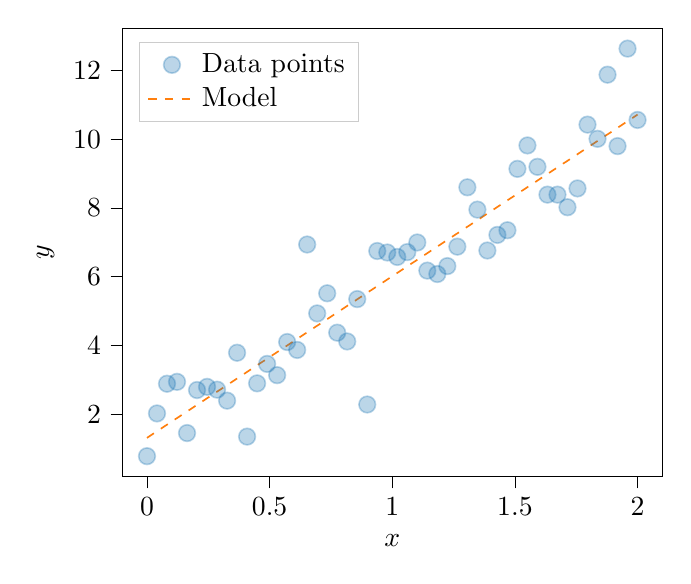
\begin{tikzpicture}

\definecolor{color0}{rgb}{0.12156862745098,0.466666666666667,0.705882352941177}
\definecolor{color1}{rgb}{1,0.498039215686275,0.0549019607843137}

\begin{axis}[
legend cell align={left},
legend style={at={(0.03,0.97)}, anchor=north west, draw=white!80.0!black},
tick align=outside,
tick pos=left,
x grid style={white!69.01960784313725!black},
xlabel={\(\displaystyle x\)},
xmin=-0.1, xmax=2.1,
xtick style={color=black},
y grid style={white!69.01960784313725!black},
ylabel={\(\displaystyle y\)},
ymin=0.189691314741281, ymax=13.2275451881467,
ytick style={color=black}
]
\addplot [semithick, color0, opacity=0.3, mark=*, mark size=3, mark options={solid}, only marks]
table {%
0 0.782321036259711
0.0408163265306122 2.02553698724508
0.0816326530612245 2.88944107434522
0.122448979591837 2.9441089401904
0.163265306122449 1.45446115861605
0.204081632653061 2.70601699452992
0.244897959183673 2.7982512222147
0.285714285714286 2.71629909502484
0.326530612244898 2.39701880091228
0.36734693877551 3.79022493810844
0.408163265306122 1.35119102451724
0.448979591836735 2.89995525231638
0.489795918367347 3.46588448890362
0.530612244897959 3.13807770245367
0.571428571428571 4.10165214881394
0.612244897959184 3.87191188228207
0.653061224489796 6.93747854025376
0.693877551020408 4.93419024396974
0.73469387755102 5.51939983211762
0.775510204081633 4.37400943826881
0.816326530612245 4.1182971232151
0.857142857142857 5.35068291521086
0.897959183673469 2.28475568552761
0.938775510204082 6.74884697743513
0.979591836734694 6.70523587752215
1.02040816326531 6.57618137004175
1.06122448979592 6.71705069578529
1.10204081632653 6.996893350413
1.14285714285714 6.17875600565952
1.18367346938776 6.07945940365117
1.22448979591837 6.31007415953039
1.26530612244898 6.87573766947214
1.30612244897959 8.60141360064448
1.3469387755102 7.95211502739419
1.38775510204082 6.76291691592648
1.42857142857143 7.21674035376784
1.46938775510204 7.35299111436777
1.51020408163265 9.1378267173966
1.55102040816327 9.81891528374901
1.59183673469388 9.19692453406167
1.63265306122449 8.38820874313926
1.6734693877551 8.38824299233666
1.71428571428571 8.02206563560459
1.75510204081633 8.5686819592157
1.79591836734694 10.4246000692698
1.83673469387755 10.0105872616746
1.87755102040816 11.8767022910241
1.91836734693878 9.79931624148078
1.95918367346939 12.6349154666283
2 10.56063787528
};
\addlegendentry{Data points}
\addplot [semithick, color1, dashed]
table {%
0 1.3144746950758
0.0408163265306122 1.50633548639334
0.0816326530612245 1.69819627771087
0.122448979591837 1.89005706902841
0.163265306122449 2.08191786034594
0.204081632653061 2.27377865166347
0.244897959183673 2.46563944298101
0.285714285714286 2.65750023429854
0.326530612244898 2.84936102561608
0.36734693877551 3.04122181693361
0.408163265306122 3.23308260825115
0.448979591836735 3.42494339956868
0.489795918367347 3.61680419088621
0.530612244897959 3.80866498220375
0.571428571428571 4.00052577352128
0.612244897959184 4.19238656483882
0.653061224489796 4.38424735615635
0.693877551020408 4.57610814747388
0.73469387755102 4.76796893879142
0.775510204081633 4.95982973010895
0.816326530612245 5.15169052142649
0.857142857142857 5.34355131274402
0.897959183673469 5.53541210406156
0.938775510204082 5.72727289537909
0.979591836734694 5.91913368669662
1.02040816326531 6.11099447801416
1.06122448979592 6.30285526933169
1.10204081632653 6.49471606064923
1.14285714285714 6.68657685196676
1.18367346938776 6.8784376432843
1.22448979591837 7.07029843460183
1.26530612244898 7.26215922591936
1.30612244897959 7.4540200172369
1.3469387755102 7.64588080855443
1.38775510204082 7.83774159987197
1.42857142857143 8.0296023911895
1.46938775510204 8.22146318250703
1.51020408163265 8.41332397382457
1.55102040816327 8.6051847651421
1.59183673469388 8.79704555645964
1.63265306122449 8.98890634777717
1.6734693877551 9.1807671390947
1.71428571428571 9.37262793041224
1.75510204081633 9.56448872172977
1.79591836734694 9.75634951304731
1.83673469387755 9.94821030436484
1.87755102040816 10.1400710956824
1.91836734693878 10.3319318869999
1.95918367346939 10.5237926783174
2 10.715653469635
};
\addlegendentry{Model}
\end{axis}

\end{tikzpicture}
  %}
  \caption{Example of linear regression applied to a simple data set of a single
    input variable. The regression tries to filter away the noise and find the
    most likely actual trend line.}
  \label{fig:linear-regression-example}
\end{figure}


We assume that the true underlying process, $f_{\valpha}(\vx)$, that generated
$\mathcal{D}$ is linear in the inputs $\vx$. For simplicity, we will also
assume that the outputs are scalar, $\vy \defeq y$. That is, we assume the data
was generated in the following way:
\begin{align}
  y_i = f_{\valpha}(\vx_i) + \epsilon = \vx^T\valpha + \epsilon
\end{align}
where $\valpha$ is a column vector of coefficients, and
$\epsilon\sim\mathcal{N}(0, \sigma^2)$ is normally distributed noise with zero
mean and variance $\sigma^2$, introduced via measurement inaccuracy
etc.\footnote{Note that this definition implies that $f_{\valpha}$
  has zero intercept, i.e. $f_{\valpha}(\vb{0}) = 0$. We can easily work around
  that, however, by adding a constant element to every input vector, i.e. let
  $\vx' \defeq (1\ \ \vx)$ be the new inputs. The second option is to simply
  center the data beforehand, by subtracting the mean $\overline y =
  \flatfrac{1}{n}\sum_{i=1}^n y_i$ from every $y_i$, and then optionally revert
  back whenever needed.}

\subsubsection{Model}

Based on the above assumption, we propose the following model:

\begin{align}
\hat f_{\hat\valpha}(\vx) &= \vx^T\hat\valpha.
\end{align}
Ideally we want to learn $\hat\valpha$ from the data such that
$\hat\valpha\simeq\valpha$.

\subsubsection{Cost Function}

In order to quantify which $\hat\valpha$ is optimal, we need metric to compare
by. There are several conceivable choices here, many of which might lead us to
the correct $\valpha$. Most common, at least in this case, is to use the
so-called Mean Square Error (MSE):

\begin{align}
  \mathcal{C}_\text{MSE}(\hat f_{\hat\valpha}; \mathcal{D}) &= \frac{1}{n}\sum_{i=1}^n \abs{\hat f_{\hat\valpha}(\vx_i) - y_i}^2.
\end{align}
The ``learning'' task is now expressed simply as the following optimization problem:
\begin{align}
  \label{eq:mse-optimization-problem-example}
  \hat\valpha = \argmin_{\valpha'}\,\mathcal{C}_\text{MSE}(\hat f_{\valpha'}; \mathcal{D})
\end{align}

\subsubsection{Optimization}

With data, model and cost function defined, the last step is to
solve~\cref{eq:mse-optimization-problem-example}. While this can in general be a
hard task (more on this in \cref{sec:ml-optimization}), we can
actually do this particular exercise analytically with some rather simple linear algebra. Skipping
the derivation, we get the following solution:
\begin{align}
  \hat\valpha = \qty(\vX^T\vX)^{-1}\vX\vy,
\end{align}
where $\vX = (\vx_1, \vx_2\,\dots\vx_n)^T$ is the matrix with inputs laid out in
rows, and $\vy$ is the column vector of all outputs.

\subsubsection{Regularization}

Often times it turns out to be useful to add an extra term to the cost function
that depends on the size of the parameters $\hat\valpha$. This typically takes
the following form:

\begin{align}
  \mathcal{C}(\hat f_{\hat\valpha};\mathcal{D}) &=   \mathcal{C}_\text{MSE}(\hat f_{\hat\valpha};\mathcal{D}) + \gamma\norm{\hat\valpha}_p^p,
\end{align}
where $\norm{\cdot}_p$ is the $L^p$ norm, and $\gamma$ is a parameter
we set to control the degree of regularization (typically $\gamma\ll 1$). Most
used are $p=1$ (called the LASSO loss) and $p=2$ (called the Ridge loss).

The motivation for why we might want to do this is as follows: Imagine we have
data set with $\vx_i = (x_i, 2x_i)$, that is to say we have two variables per
data point, but the two variables are directly correlated. Lastly, assume that
$y_i = 3x_i$ is the underlying function. Without any regularization, all of the
following models are equally good:

\begin{align}
  \hat\valpha^{(1)} = (3, 0),\ \hat\valpha^{(2)} = (1, 1),\ \hat\valpha^{(3)} = (-997, 500)
\end{align}
The problem is that without regularization, this particular
optimization problem ill-formed, and does not have a unique solution. While all
of the above give perfect reconstruction of the data, solutions like
$\valpha^{(3)}$ yield strange interpretations. According to this model, the
output is strongly negatively correlated with $x_1$, in complete contradiction
with the underlying truth.

While this particular example is very contrived, the point should be clear: In
some cases, depending on both the data and what model we choose, the model might
be too flexible for the task at hand. This is generally referred to as the
problem of \emph{overfitting}, and can lead to strange behavior. The opposite
problem called \emph{underfitting} refers to the case where the model is too
constrained, e.g. trying to fit a first order polynomial to
quadratic data.

\section{Gradient Based Optimization}
\label{sec:ml-optimization}

Most supervised learning tasks rely on a gradient based optimization strategy,
with the umbrella name \emph{Gradient Decent} (GD).
These methods can be summarized as follows: We want to find $\vx^*$ such that\footnote{For maximization, simply minimize $-f(\vx)$. }

\begin{align}
  \vx^* = \argmin_{\vx} g(\vx),
\end{align}
for some function $g$ that should be minimized.
Solve this by starting at some initial guess $\vx^{(0)}$ and improving it by
iterating the following recurrence relation:

\begin{align}
  \label{eq:gradient-decent-definition}
  \vx^{(n+1)} &= \vx^{(n)} + \Delta \vx^{(n)} = \vx^{(n)} - \gamma \grad{f}(\vx^{(n)})
\end{align}
where $\gamma$ is a suitably chosen number, typically $\gamma \ll 1$. In the
limit $n\to\infty$ (if $\gamma$ is small enough), this will converge to a minimum
for $f$.

When $f=\mathcal{C}(\hat f_{\hat\valpha}; \mathcal{D})$ we have some choice in
exactly how we should compute $\grad{\mathcal{C}}$. We could compute the cost
for the entire data set, or just a single data point. These
two options are referred to as Gradient Decent (GD) and Stochastic Gradient
Decent (SGD), respectively. The latter is most often used because it is less
computationally expensive for large data sets.

We have various ways of extending the basic algorithm in
\cref{eq:gradient-decent-definition}, some of which we will mention here.

\subsection{Fixed Learning Rate}

This is the version presented in \cref{eq:gradient-decent-definition}, in where
$\gamma$ is chosen in advance and remains fixed throughout all iterations.

\begin{itemize}
\item Pros:
  \begin{itemize}
  \item Easy to implement
  \end{itemize}
\item Cons:
  \begin{itemize}
  \item If $\gamma$ is to large it can lead to divergence or inaccurate results
  \item If $\gamma$ is to small we have a higher chance of getting stuck in small, local minima.
  \item If $\gamma$ is small we will need many iterations before convergence
  \end{itemize}
\end{itemize}

\subsection{Momentum}

\section{Neural Networks}

\subsection{Nodes and Connections}

\subsection{Activation Functions}

\subsection{Backpropagation}


\end{document}
